\section{Theory}

\subsection{Bipolar Junction Transistor (BJT)}
The Bipolar Junction Transistor (BJT) is essentially a combination of two PN junction diodes.  According to the order in which the diodes are connected, we have npn and pnp transistors. The emitter region is much smaller than the collector and much more strongly doped while the base is very thing and very lightly doped. A large collector is needed since it should have more surface area for dissipating the power generated there.\\[0.3cm]
\begin{figure}[H]
    \centering


    \tikzset{every picture/.style={line width=0.75pt}} %set default line width to 0.75pt        

    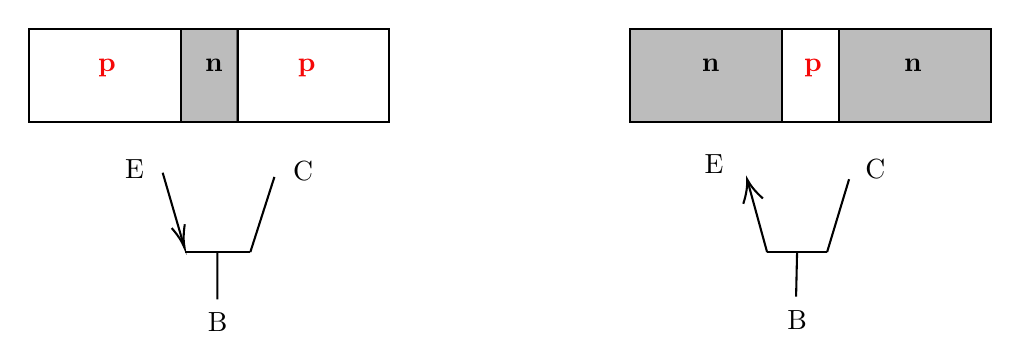
\begin{tikzpicture}[x=0.75pt,y=0.75pt,yscale=-1,xscale=1]
    %uncomment if require: \path (0,226); %set diagram left start at 0, and has height of 226
    
    %Shape: Rectangle [id:dp45633474700626153] 
    \draw  [fill={rgb, 255:red, 255; green, 255; blue, 255 }  ,fill opacity=1 ] (95.6,52) -- (168.81,52) -- (168.81,96.74) -- (95.6,96.74) -- cycle ;
    %Shape: Rectangle [id:dp14383516673441366] 
    \draw  [fill={rgb, 255:red, 255; green, 255; blue, 255 }  ,fill opacity=1 ] (195.79,52) -- (269,52) -- (269,96.74) -- (195.79,96.74) -- cycle ;
    %Shape: Rectangle [id:dp555436172774842] 
    \draw  [fill={rgb, 255:red, 155; green, 155; blue, 155 }  ,fill opacity=0.67 ] (168.81,52) -- (196.26,52) -- (196.26,96.74) -- (168.81,96.74) -- cycle ;
    %Shape: Rectangle [id:dp25579750012111335] 
    \draw  [fill={rgb, 255:red, 155; green, 155; blue, 155 }  ,fill opacity=0.67 ] (385.38,52) -- (458.59,52) -- (458.59,96.74) -- (385.38,96.74) -- cycle ;
    %Shape: Rectangle [id:dp7671828884714951] 
    \draw  [fill={rgb, 255:red, 155; green, 155; blue, 155 }  ,fill opacity=0.67 ] (486.04,52) -- (559.25,52) -- (559.25,96.74) -- (486.04,96.74) -- cycle ;
    %Shape: Rectangle [id:dp5338560444707424] 
    \draw  [fill={rgb, 255:red, 255; green, 255; blue, 255 }  ,fill opacity=1 ] (458.59,52) -- (486.04,52) -- (486.04,96.74) -- (458.59,96.74) -- cycle ;
    %Straight Lines [id:da24796501054461773] 
    \draw    (170.7,159.64) -- (202.37,159.64) ;
    %Straight Lines [id:da6481562502442813] 
    \draw    (170.14,155.72) -- (160.15,121.4) ;
    \draw [shift={(170.7,157.64)}, rotate = 253.76] [color={rgb, 255:red, 0; green, 0; blue, 0 }  ][line width=0.75]    (10.93,-3.29) .. controls (6.95,-1.4) and (3.31,-0.3) .. (0,0) .. controls (3.31,0.3) and (6.95,1.4) .. (10.93,3.29)   ;
    %Straight Lines [id:da7575975492052729] 
    \draw    (202.37,159.64) -- (213.98,123.4) ;
    %Straight Lines [id:da35919367940892855] 
    \draw    (451.35,159.64) -- (480.25,159.64) ;
    %Straight Lines [id:da5671054714723539] 
    \draw    (451.35,159.64) -- (442.24,126.45) ;
    \draw [shift={(441.71,124.52)}, rotate = 74.66] [color={rgb, 255:red, 0; green, 0; blue, 0 }  ][line width=0.75]    (10.93,-4.9) .. controls (6.95,-2.3) and (3.31,-0.67) .. (0,0) .. controls (3.31,0.67) and (6.95,2.3) .. (10.93,4.9)   ;
    %Straight Lines [id:da2022169589051811] 
    \draw    (480.25,159.64) -- (490.85,124.52) ;
    %Straight Lines [id:da04159202121636396] 
    \draw    (186.53,159.64) -- (186.5,182.37) ;
    %Straight Lines [id:da31155623971098534] 
    \draw    (465.8,159.64) -- (465.32,181.06) ;
    
    % Text Node
    \draw (418.48,65.31) node [anchor=north west][inner sep=0.75pt]   [align=left] {\textbf{n}};
    % Text Node
    \draw (515.86,65.37) node [anchor=north west][inner sep=0.75pt]   [align=left] {\textbf{n}};
    % Text Node
    \draw (179.15,65.31) node [anchor=north west][inner sep=0.75pt]  [color={rgb, 255:red, 0; green, 0; blue, 0 }  ,opacity=1 ] [align=left] {\textbf{n}};
    % Text Node
    \draw (223.73,65.31) node [anchor=north west][inner sep=0.75pt]   [align=left] {\textcolor[rgb]{0.96,0.03,0.03}{\textbf{p}}};
    % Text Node
    \draw (127.53,65.31) node [anchor=north west][inner sep=0.75pt]   [align=left] {\textcolor[rgb]{0.96,0.03,0.03}{\textbf{p}}};
    % Text Node
    \draw (467.75,65.31) node [anchor=north west][inner sep=0.75pt]   [align=left] {\textcolor[rgb]{0.96,0.03,0.03}{\textbf{p}}};
    % Text Node
    \draw (140.52,113.41) node [anchor=north west][inner sep=0.75pt]   [align=left] {E};
    % Text Node
    \draw (221.55,114.53) node [anchor=north west][inner sep=0.75pt]   [align=left] {C};
    % Text Node
    \draw (180.41,187.23) node [anchor=north west][inner sep=0.75pt]   [align=left] {B};
    % Text Node
    \draw (419.74,111.17) node [anchor=north west][inner sep=0.75pt]   [align=left] {E};
    % Text Node
    \draw (459.63,186.12) node [anchor=north west][inner sep=0.75pt]   [align=left] {B};
    % Text Node
    \draw (497.26,113.41) node [anchor=north west][inner sep=0.75pt]   [align=left] {C};
    
    
    \end{tikzpicture}
    

\end{figure}

\noindent
It is a three terminal device with the terminals named as emitter, base and collector but to act as an amplifier, we need four terminals. Hence, we make one terminal common. The most commonly studied configuration is the common emitter configuration where the emmiter is common to both input and output.\\[0.3cm]
A BJT works in three modes: Active, Saturation and Cutoff Modes, according to which junction is forward or reverse biased.  
\subsection{Common Emitter Configuration of BJT}

\begin{figure}[H]    
    \centering
    \begin{circuitikz}[american voltages ]
        \draw
        % Transistor
        (0,0) node[npn, anchor=E, tr circle, fill = cyan!40!white] (Q) {}
        (Q.B) node[above left] {B}
        (Q.C) node[right] {C}
        (Q.E) node[below left] {E}
        % Base resistor
        (Q.B) -- (-2,0.75) to[R, l=$\mathrm{R_B}$] (-4,0.75) to [rmeter, t = $\mathrm{\mu A}$,fill = yellow!60!white]  (-6,0.75)
        to[battery, v_=$\mathrm{V_{BB}}$] (-6,-2) -- (0,-2)
    
        % Collector resistor
        (Q.C) -- (0,2) to[R, l=$\mathrm{R_C}$] (4,2)
        to [rmeter, t= $\mathrm{mA}$, fill = yellow!60!white] (5,2) -- (7,2)
        to [battery, v=$\mathrm{V_{CC}}$] (7,-2) -- (0,-2) 
    
        % Ground connection
        (Q.E) -- (0,-2) node[ground] {};
    \end{circuitikz}   
    \caption{Circuit diagram of a common emitter configuration of a NPN transistor}  
\end{figure}


The above figure shows the common emitter configuration of the transistor. From the figure, we can see: 
$$\mathrm{I_E = I_B+ I_C}$$
Normally when used as an amplifier,
the base emitter junction is kept in forward bias and the collector base junction is kept
in reverse bias. So, due to the forward bias of the base emitter junction electrons go
from emitter to the base, this electrons get affected by the reverse bias of the collector
base junction and as the base is very thin and lightly doped most of the electrons go
to the collector. So the emitter current is almost equal to the collector current. We define two parameters $\beta$ and $\alpha$ for the transistor as follows:
$$\beta = \mathrm{\frac{I_C}{I_B}}$$
$$\alpha = \mathrm{\frac{I_C}{I_E}}$$
From this, we get a relation between $\alpha$ and $\beta$ as:
$$\alpha = \mathrm{\frac{\beta}{1+\beta}} \implies \beta = \frac{\alpha}{1-\alpha} $$
Generally $\beta$ is much greater than 1 while $\alpha$ is very close to but less than 1 .\\[0.3cm]
In the CE configuration the input current and voltage are $\mathrm{I_B}$ and $\mathrm{V_{BE}}$, while the output current and voltage are $\mathrm{I_C}$ and $\mathrm{V_{CE}}$. Thus, for the input characteristics, we plot $\mathrm{I_B}$ vs $\mathrm{V_{BE}}$ and for the output characteristics, we plot $\mathrm{I_C}$ vs $\mathrm{V_{CE}}$.\\[0.2cm]